\chapter{Capa de la nube}
En este apartado se van a especificar los requisitos funciones y no funcionales del sistema, la estructura y desarrollo tanto del back-end como del front-end, y el despliegue del sistema. Esta capa tiene almacenada por un lado la parte de la base de datos, back-end del sistema, y la interfaz gráfica, front-end del sistema. 

\section{Análisis}
En esta primera fase se realiza un análisis del sistema a desarrollar. En primer lugar, se realiza un estudio de la funcionalidad que debe contener el sistema, realizando un diagrama de casos de uso y una descripción de los casos de uso subyacentes a éste. En segundo lugar, se indican los requisitos no funcionales del sistema y de qué forma se consiguen cumplir en cada caso.

\subsection{Requisitos funcionales}
La etapa de análisis del software es fundamental a la hora de desarrollar software ya que problemas en esta primera fase de análisis pueden tener consecuencias nefastas una vez que se encuentra el sistema en fase de implementación.

Con el objetivo de realizar un correcto análisis y diseño del sistema nace UML (Lenguaje de modelado de sistemas de software más conocido y utilizado en la actualidad), se trata de un estándar de modelado de software, respaldado por la OMG (Consorcio formado en 1989 dedicado al cuidado y el establecimiento de diversos estándares de tecnologías orientadas a objetos).

UML proporciona una serie de herramientas útiles para la realización de las fases de análisis, diseño y documentación del software. Concretamente, en esta sección se usan los diagramas de caso de uso.

Los diagramas de casos de uso nacen con el objetivo de recoger la interacción entre un sistema y los usuarios que pueden interactuar con éste. Estos sistemas están formados por lo tanto por casos de uso, actores y relaciones entre ellos.

En la Figura 7.1 se muestra el diagrama de casos de uso de la funcionalidad incluida en el sistema. En total el sistema contará con la participación de 3 roles de usuarios. Estos usuarios son los siguientes.

\begin{itemize}
    \item \textbf{Usuario no logueado:} Es un usuario que no ha iniciado sesión. Puede hacer acciones muy limitadas, o iniciar sesión para obtener más acciones.
    \item \textbf{Usuario logueado como usuario estándar:} Se trata del usuario que ha iniciado correctamente sesión en el sistema y tiene acceso a la funcionalidad principales de éste. Una vez cierra sesión, vuelve a ser un usuario no logueado.
    \item \textbf{Usuario logueado como usuario administrador:} Se trata del usuario que ha iniciado correctamente sesión en el sistema y tiene acceso a la funcionalidad principales de éste como el usuario estándar, y algunas más, como gestión de usuarios, de variables y de datos en la base de datos, entre otras. Es el único usuario que puede acceder a todos las funcionalidades del sistema. Una vez cierra sesión, vuelve a ser un usuario no logueado.
\end{itemize}

A continuación, se realiza una descripción de los casos de uso, mostrando los siguientes campos en cada uno.

\begin{itemize}
    \item \textbf{Resumen:} Pequeña descripción de la funcionalidad que se lleva a cabo en el caso de uso. 
    \item \textbf{Sistemas:} Sistema que implementa el caso de uso. 
    \item \textbf{Condiciones previas:} Estado del usuario en el sistema previo al comienzo del caso de uso. 
    \item \textbf{Flujo de eventos:} Secuencia de acciones por parte del sistema y actor en la ejecución del caso de uso.
    \item \textbf{Condiciones de salida:} Estado del sistema y actor una vez finalizada la ejecución de la funcionalidad recogida en el caso de uso.
    \item \textbf{Alternativas:} Posibles caminos alternativos en la ejecución del caso de uso. 
\end{itemize}

\begin{landscape}
    \begin{figure}[h]
        \centering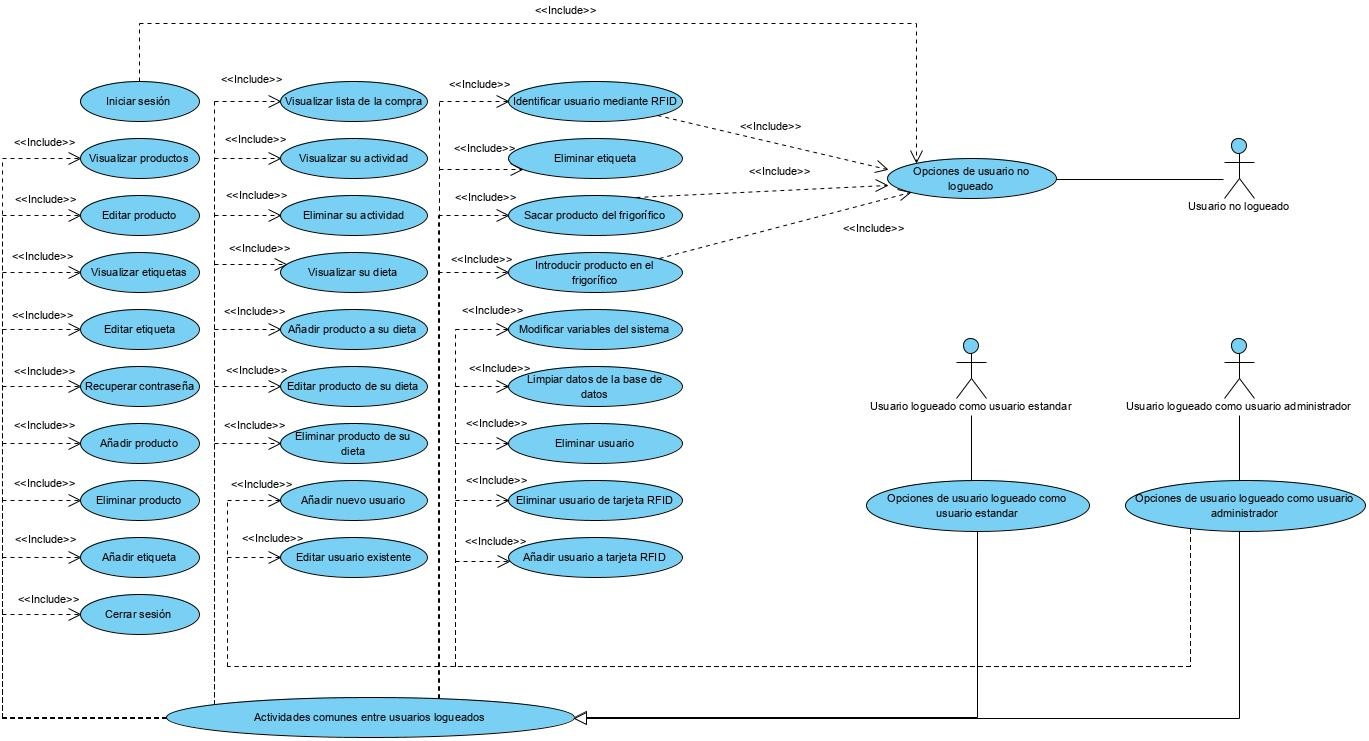
\includegraphics[width=\hsize]{capitulos/capitulo8/requisitos.jpg}
        \caption{Diagrama de casos de uso del sistema.}
        \label{img_gantt}
    \end{figure}
\end{landscape}

\begin{longtable}{|p{.90\textwidth}|}
\hline
 \rowcolor[gray]{.5}
 \color{white}\textbf{Requisito 1: Iniciar sesión} \\
\hline
\endfirsthead
\endhead
\hline \multicolumn{1}{r}{\textit{Continua en la siguiente página}} \\
\endfoot
\endlastfoot
    \rowcolor[gray]{.9}
     \textbf{Resumen}  \\
     \hline
     El usuario debe iniciar sesión para poder acceder al sistema. \\
     \hline
     \rowcolor[gray]{.9}
     \textbf{Actores principales} \\
     \hline
     Usuario no logueado. \\
     \hline
     \rowcolor[gray]{.9}
     \textbf{Sistema} \\
     \hline
     Aplicación web. \\
     \hline
     \rowcolor[gray]{.9}
     \textbf{Condiciones previas} \\
     \hline
     El usuario se encuentra en la página de inicio de sesión en el sistema. \\
     \hline
     \rowcolor[gray]{.9}
     \textbf{Flujo de eventos} \\
     \hline
      \begin{itemize}
         \item El sistema muestra un formulario de inicio de sesión.
         \item El usuario introduce el email/usuario y contraseña requeridos.
         \item El sistema valida los datos y permite al usuario entrar en el sistema.
     \end{itemize} \\
     \hline
     \rowcolor[gray]{.9}
     \textbf{Condiciones de salida} \\
     \hline
     El sistema permite al usuario entrar en el sistema localizándose en la página principal de éste. \\
     \hline
     \rowcolor[gray]{.9}
     \textbf{Alternativas}  \\
     \hline
      \begin{itemize}
        \item El email/usuario introducido para recuperar la contraseña no existe. Se muestra un mensaje con el error.
        \item El usuario ha introducido una contraseña errónea. Se muestra un mensaje con el error.
     \end{itemize} \\
     \hline
\end{longtable}

\begin{longtable}{|p{0.90\textwidth}|}
\hline
\rowcolor[gray]{.5}
 \color{white}\textbf{Requisito 2: Cerrar sesión} \\
\hline
\endfirsthead
\endhead
\hline \multicolumn{1}{r}{\textit{Continua en la siguiente página}} \\
\endfoot
\endlastfoot
    \rowcolor[gray]{.9}
     \textbf{Resumen} \\
     \hline
     El usuario cierra sesión en el sistema. \\
     \hline
     \rowcolor[gray]{.9}
     \textbf{Actores principales} \\
     \hline
     Usuario logueado con usuario estándar y con usuario administrador. \\
     \hline
     \rowcolor[gray]{.9}
     \textbf{Sistema} \\
     \hline
     Aplicación web. \\
     \hline
     \rowcolor[gray]{.9}
     \textbf{Condiciones previas} \\
     \hline
      El usuario se encuentra en cualquier página del sistema.\\
     \hline
     \rowcolor[gray]{.9}
     \textbf{Flujo de eventos} \\
     \hline
      \begin{itemize}
         \item El sistema muestra constantemente un botón para cerrar sesión.
         \item El usuario pulsa ese botón y confirma con un segundo clic en un pop-up.
         \item El sistema obtiene el usuario que está logueado de las cookies del navegador y cierra la sesión de éste.
     \end{itemize} \\
     \hline
     \rowcolor[gray]{.9}
     \textbf{Condiciones de salida} \\
     \hline
     El sistema termina cerrando la sesión del usuario logueado y el usuario se encuentra en la ventana de inicio de sesión. \\
     \hline
     \rowcolor[gray]{.9}
     \textbf{Alternativas}  \\
     \hline
     Ninguna. \\
     \hline
\end{longtable}

\begin{longtable}{|p{0.90\textwidth}|}
\hline
\rowcolor[gray]{.5}
 \color{white}\textbf{Requisito 3: Recuperar contraseña} \\
\hline
\endfirsthead
\endhead
\hline \multicolumn{1}{r}{\textit{Continua en la siguiente página}} \\
\endfoot
\endlastfoot
    \rowcolor[gray]{.9}
     \textbf{Resumen} \\
     \hline
     El usuario puede recuperar el acceso a su cuenta introduciendo sus datos y validando su identidad con una clave de seguridad que se enviará a su correo para validad su identidad. \\
     \hline
     \rowcolor[gray]{.9}
     \textbf{Actores principales} \\
     \hline
     Usuario no logueado. \\
     \hline
     \rowcolor[gray]{.9}
     \textbf{Sistema} \\
     \hline
     Aplicación web. \\
     \hline
     \rowcolor[gray]{.9}
     \textbf{Condiciones previas} \\
     \hline
     El usuario se encuentra en la página de recuperar contraseña en el sistema. \\
     \hline
     \rowcolor[gray]{.9}
     \textbf{Flujo de eventos}  \\
     \hline
      \begin{itemize}
         \item El sistema muestra un formulario donde el usuario introduce su email/usuario.
         \item El sistema busca al usuario y envía un correo a él con una clave de seguridad y reenvía al usuario a otro formulario para introducir la clave de seguridad del correo y la nueva contraseña escrita dos veces para asegurar de que no se equivoca.
         \item El usuario introduce clave de seguridad y la nueva contraseña dos veces.
         \item El sistema comprueba que esa clave de seguridad coincide con la guardada en el usuario y comprueba que las dos contraseñas introducidas son iguales. Si es así, guarda la contraseña nueva en el usuario.
     \end{itemize} \\
     \hline
     \rowcolor[gray]{.9}
     \textbf{Condiciones de salida} \\
     \hline
     El sistema ha cambiado la clave del usuario y éste puede acceder al sistema con la clave nueva. \\
     \hline
     \rowcolor[gray]{.9}
     \textbf{Alternativas}  \\
     \hline
      \begin{itemize}
         \item El usuario introducido no existe. Se muestra un mensaje con el error.
         \item El usuario ha introducido dos contraseñas diferentes. Se muestra un mensaje con el error.
         \item El usuario ha introducido una clave de seguridad errónea. Se muestra un mensaje con el error.
     \end{itemize} \\
     \hline
\end{longtable}

\begin{longtable}{|p{0.90\textwidth}|}
\hline
 \rowcolor[gray]{.5}
 \color{white}\textbf{Requisito 4: Visualizar productos.} \\
\hline
\endfirsthead
\endhead
\hline \multicolumn{1}{r}{\textit{Continua en la siguiente página}} \\
\endfoot
\endlastfoot
    \rowcolor[gray]{.9}
     \textbf{Resumen} \\
     \hline
     El usuario puede visualizar los diferentes productos del frigorífico ordenados por categorías y la cantidad de cada producto, además de poner interactuar con ellos para editarlos o eliminarlos. \\
     \hline
     \rowcolor[gray]{.9}
     \textbf{Actores principales} \\
     \hline
     Usuario logueado con usuario estándar o con usuario administrador. \\
     \hline
     \rowcolor[gray]{.9}
     \textbf{Sistema} \\
     \hline
     Aplicación web. \\
     \hline
     \rowcolor[gray]{.9}
     \textbf{Condiciones previas} \\
     \hline
     El usuario se encuentra en la página de productos del sistema. \\
     \hline
     \rowcolor[gray]{.9}
     \textbf{Flujo de eventos}  \\
     \hline
      \begin{itemize}
         \item El usuario accede a la página de los productos.
         \item El sistema obtiene todos los productos de la base de datos y los muestra ordenados por categoría.
     \end{itemize} \\
     \hline
     \rowcolor[gray]{.9}
     \textbf{Condiciones de salida} \\
     \hline
     El sistema ha cargado los productos y el usuario puede visualizarlos. \\
     \hline
     \rowcolor[gray]{.9}
     \textbf{Alternativas}  \\
     \hline
      Ninguna.\\
     \hline
\end{longtable}

\begin{longtable}{|p{0.90\textwidth}|}
\hline
 \rowcolor[gray]{.5}
 \color{white}\textbf{Requisito 5: Añadir producto.} \\
\hline
\endfirsthead
\endhead
\hline \multicolumn{1}{r}{\textit{Continua en la siguiente página}} \\
\endfoot
\endlastfoot
    \rowcolor[gray]{.9}
     \textbf{Resumen} \\
     \hline
     El usuario crea un producto nuevo para introducirlo en el frigorífico y tener un seguimiento de éste desde el sistema. \\
     \hline
     \rowcolor[gray]{.9}
     \textbf{Actores principales} \\
     \hline
     Usuario logueado con usuario estándar o con usuario administrador. \\
     \hline
     \rowcolor[gray]{.9}
     \textbf{Sistema} \\
     \hline
     Aplicación web. \\
     \hline
     \rowcolor[gray]{.9}
     \textbf{Condiciones previas} \\
     \hline
     El usuario se encuentra en la página de productos del sistema. \\
     \hline
     \rowcolor[gray]{.9}
     \textbf{Flujo de eventos}  \\
     \hline
      \begin{itemize}
         \item El usuario despliega el formulario e introduce el contenido.
         \item El sistema comprueba que no existe el producto ya. Si no existe, lo crea y devuelve un mensaje al usuario.
     \end{itemize} \\
     \hline
     \rowcolor[gray]{.9}
     \textbf{Condiciones de salida} \\
     \hline
     El sistema ha guardado el producto y el usuario puede visualizarlo en la lista, además de recibir un mensaje de confirmación. \\
     \hline
     \rowcolor[gray]{.9}
     \textbf{Alternativas}  \\
     \hline
      \begin{itemize}
         \item El producto a añadir ya existe. Se muestra un mensaje con el error.
     \end{itemize} \\
     \hline
\end{longtable}

\begin{longtable}{|p{0.90\textwidth}|}
\hline
 \rowcolor[gray]{.5}
 \color{white}\textbf{Requisito 6: Editar producto.} \\
\hline
\endfirsthead
\endhead
\hline \multicolumn{1}{r}{\textit{Continua en la siguiente página}} \\
\endfoot
\endlastfoot
    \rowcolor[gray]{.9}
     \textbf{Resumen} \\
     \hline
     El usuario puede modificar parámetros de un producto en especifico una vez creado. \\
     \hline
     \rowcolor[gray]{.9}
     \textbf{Actores principales} \\
     \hline
     Usuario logueado con usuario estándar o con usuario administrador. \\
     \hline
     \rowcolor[gray]{.9}
     \textbf{Sistema} \\
     \hline
     Aplicación web. \\
     \hline
     \rowcolor[gray]{.9}
     \textbf{Condiciones previas} \\
     \hline
     El usuario se encuentra en la página de productos del sistema. \\
     \hline
     \rowcolor[gray]{.9}
     \textbf{Flujo de eventos}  \\
     \hline
      \begin{itemize}
         \item El usuario hace clic en el botón de editar situado debajo del producto a modificar.
         \item El sistema muestra un formulario con los datos del producto con la posibilidad de ser modificados por el usuario.
         \item El usuario modifica los parámetros que el desee y envía el formulario.
         \item El sistema comprueba que parámetros se han modificado en el formulario y los modifica en la base de datos y devuelve un mensaje de confirmación.
     \end{itemize} \\
     \hline
     \rowcolor[gray]{.9}
     \textbf{Condiciones de salida} \\
     \hline
     El sistema ha guardado el producto y el usuario puede visualizarlo en la lista, además de recibir un mensaje de confirmación. \\
     \hline
     \rowcolor[gray]{.9}
     \textbf{Alternativas}  \\
     \hline
      \begin{itemize}
         \item El producto modificado se le ha puesto un nombre de otro producto que ya existe. Se muestra un mensaje con el error.
     \end{itemize} \\
     \hline
\end{longtable}

\begin{longtable}{|p{0.90\textwidth}|}
\hline
 \rowcolor[gray]{.5}
 \color{white}\textbf{Requisito 7: Eliminar producto.} \\
\hline
\endfirsthead
\endhead
\hline \multicolumn{1}{r}{\textit{Continua en la siguiente página}} \\
\endfoot
\endlastfoot
    \rowcolor[gray]{.9}
     \textbf{Resumen} \\
     \hline
     El usuario puede eliminar un producto en específico. \\
     \hline
     \rowcolor[gray]{.9}
     \textbf{Actores principales} \\
     \hline
     Usuario logueado con usuario estándar o con usuario administrador. \\
     \hline
     \rowcolor[gray]{.9}
     \textbf{Sistema} \\
     \hline
     Aplicación web. \\
     \hline
     \rowcolor[gray]{.9}
     \textbf{Condiciones previas} \\
     \hline
     El usuario se encuentra en la página de productos del sistema. \\
     \hline
     \rowcolor[gray]{.9}
     \textbf{Flujo de eventos}  \\
     \hline
      \begin{itemize}
         \item El usuario hace clic en el botón de eliminar situado debajo del producto y confirma con un doble clic en un mensaje que se muestra de confirmación.
         \item El sistema obtiene el ID del producto y lo elimina de la base de datos y recarga los productos de la lista para visualizarlos sin el producto eliminado.
     \end{itemize} \\
     \hline
     \rowcolor[gray]{.9}
     \textbf{Condiciones de salida} \\
     \hline
     El sistema ha eliminado el producto y el usuario puede visualizarlo en la lista. \\
     \hline
     \rowcolor[gray]{.9}
     \textbf{Alternativas}  \\
     \hline
      Ninguna.\\
     \hline
\end{longtable}

\begin{longtable}{|p{0.90\textwidth}|}
\hline
 \rowcolor[gray]{.5}
 \color{white}\textbf{Requisito 8: Visualizar etiquetas.} \\
\hline
\endfirsthead
\endhead
\hline \multicolumn{1}{r}{\textit{Continua en la siguiente página}} \\
\endfoot
\endlastfoot
     \rowcolor[gray]{.9}
     \textbf{Resumen} \\
     \hline
     El usuario puede visualizar las diferentes etiquetas a añadir al frigorífico ordenadas por orden de entrada y la cantidad de cada etiqueta, además de poner interactuar con ellos para editarlas o eliminarlas. Las etiquetas mostradas son las que van a ser registradas en una tarjeta RFID para agregarla a un producto. \\
     \hline
     \rowcolor[gray]{.9}
     \textbf{Actores principales} \\
     \hline
     Usuario logueado con usuario estándar o con usuario administrador. \\
     \hline
     \rowcolor[gray]{.9}
     \textbf{Sistema} \\
     \hline
     Aplicación web. \\
     \hline
     \rowcolor[gray]{.9}
     \textbf{Condiciones previas} \\
     \hline
     El usuario se encuentra en la página de etiquetas del sistema. \\
     \hline
     \rowcolor[gray]{.9}
     \textbf{Flujo de eventos}  \\
     \hline
      \begin{itemize}
         \item El usuario accede a la página de las etiquetas.
         \item El sistema obtiene todas las etiquetas de la base de datos y las muestra ordenados por orden de entrada.
     \end{itemize} \\
     \hline
     \rowcolor[gray]{.9}
     \textbf{Condiciones de salida} \\
     \hline
     El sistema ha cargado las etiquetas y el usuario puede visualizarlas. \\
     \hline
     \rowcolor[gray]{.9}
     \textbf{Alternativas}  \\
     \hline
      Ninguna.\\
     \hline
\end{longtable}

\begin{longtable}{|p{0.90\textwidth}|}
\hline
 \rowcolor[gray]{.5}
 \color{white}\textbf{Requisito 9: Añadir etiqueta.} \\
\hline
\endfirsthead
\endhead
\hline \multicolumn{1}{r}{\textit{Continua en la siguiente página}} \\
\endfoot
\endlastfoot
    \rowcolor[gray]{.9}
     \textbf{Resumen} \\
     \hline
     El usuario crea una etiqueta nueva para introducirla en el frigorífico con el producto. \\
     \hline
     \rowcolor[gray]{.9}
     \textbf{Actores principales} \\
     \hline
     Usuario logueado con usuario estándar o con usuario administrador. \\
     \hline
     \rowcolor[gray]{.9}
     \textbf{Sistema} \\
     \hline
     Aplicación web. \\
     \hline
     \rowcolor[gray]{.9}
     \textbf{Condiciones previas} \\
     \hline
     El usuario se encuentra en la página de etiquetas del sistema. \\
     \hline
     \rowcolor[gray]{.9}
     \textbf{Flujo de eventos}  \\
     \hline
      \begin{itemize}
         \item El usuario despliega el formulario e introduce el contenido.
         \item El sistema comprueba que no existe la etiqueta ya. Si no existe, la crea y devuelve un mensaje al usuario.
     \end{itemize} \\
     \hline
     \rowcolor[gray]{.9}
     \textbf{Condiciones de salida} \\
     \hline
     El sistema ha guardado la etiqueta y el usuario puede visualizarlas en la lista, además de recibir un mensaje de confirmación. \\
     \hline
     \rowcolor[gray]{.9}
     \textbf{Alternativas}  \\
     \hline
      \begin{itemize}
         \item La etiqueta a añadir ya existe. Se muestra un mensaje con el error.
     \end{itemize} \\
     \hline
\end{longtable}

\begin{longtable}{|p{0.90\textwidth}|}
\hline
 \rowcolor[gray]{.5}
 \color{white}\textbf{Requisito 10: Editar etiqueta.} \\
\hline
\endfirsthead
\endhead
\hline \multicolumn{1}{r}{\textit{Continua en la siguiente página}} \\
\endfoot
\endlastfoot
    \rowcolor[gray]{.9}
    \textbf{Resumen} \\
     \hline
     El usuario puede modificar parámetros de una etiqueta en especifico una vez creada. \\
    \hline
    \rowcolor[gray]{.9}
    \textbf{Actores principales} \\
     \hline
     Usuario logueado con usuario estándar o con usuario administrador. \\
    \hline
    \rowcolor[gray]{.9}
    \textbf{Sistema} \\
     \hline
     Aplicación web. \\
    \hline
    \rowcolor[gray]{.9}
    \textbf{Condiciones previas} \\
     \hline
     El usuario se encuentra en la página de etiquetas del sistema. \\
    \hline
    \rowcolor[gray]{.9}
    \textbf{Flujo de eventos}  \\
     \hline
      \begin{itemize}
        \item El usuario hace clic en el botón de editar situado debajo de la etiqueta a modificar.
        \item El sistema muestra un formulario con los datos de la etiqueta con la posibilidad de ser modificados por el usuario.
        \item El usuario modificar los parámetros que el desee y envía el formulario.
        \item El sistema comprueba que parámetros se han modificado en el formulario y los modifica en la base de datos y devuelve un mensaje de confirmación.
    \end{itemize} \\
    \hline
    \rowcolor[gray]{.9}
    \textbf{Condiciones de salida} \\
     \hline
     El sistema ha guardado la etiqueta y el usuario puede visualizarla en la lista, además de recibir un mensaje de confirmación. \\
    \hline
    \rowcolor[gray]{.9}
    \textbf{Alternativas}  \\
     \hline
      Ninguna. \\
    \hline
\end{longtable}

\begin{longtable}{|p{0.90\textwidth}|}
\hline
 \rowcolor[gray]{.5}
 \color{white}\textbf{Requisito 11: Eliminar etiqueta.} \\
\hline
\endfirsthead
\endhead
\hline \multicolumn{1}{r}{\textit{Continua en la siguiente página}} \\
\endfoot
\endlastfoot
    \rowcolor[gray]{.9}
    \textbf{Resumen} \\
     \hline
     El usuario puede eliminar una etiqueta en especifico. \\
    \hline
    \rowcolor[gray]{.9}
    \textbf{Actores principales} \\
     \hline
     Usuario logueado con usuario estándar o con usuario administrador. \\
    \hline
    \rowcolor[gray]{.9}
    \textbf{Sistema} \\
     \hline
     Aplicación web. \\
    \hline
    \rowcolor[gray]{.9}
    \textbf{Condiciones previas} \\
     \hline
     El usuario se encuentra en la página de etiquetas del sistema. \\
    \hline
    \rowcolor[gray]{.9}
    \textbf{Flujo de eventos}  \\
     \hline
      \begin{itemize}
        \item El usuario hace clic en el botón de eliminar situado debajo de la etiqueta y confirma con un doble clic en un mensaje que se muestra de confirmación.
        \item El sistema obtiene el ID de la etiqueta y la elimina de la base de datos y recarga las etiqueta de la lista para visualizarlas sin la etiqueta eliminada.
    \end{itemize} \\
    \hline
    \rowcolor[gray]{.9}
    \textbf{Condiciones de salida} \\
     \hline
     El sistema ha eliminado la etiqueta y el usuario puede visualizarlo en la lista. \\
    \hline
    \rowcolor[gray]{.9}
    \textbf{Alternativas}  \\
     \hline
      Ninguna.\\
    \hline
\end{longtable}

\begin{longtable}{|p{0.90\textwidth}|}
\hline
 \rowcolor[gray]{.5}
 \color{white}\textbf{Requisito 12: Visualizar lista de la compra.} \\
\hline
\endfirsthead
\endhead
\hline \multicolumn{1}{r}{\textit{Continua en la siguiente página}} \\
\endfoot
\endlastfoot
    \rowcolor[gray]{.9}
    \textbf{Resumen} \\
     \hline
     El usuario puede visualizar los diferentes productos del frigorífico que son necesarios comprar porque están por debajo del umbral especificado en la configuración del sistema. \\
    \hline
    \rowcolor[gray]{.9}
    \textbf{Actores principales} \\
     \hline
     Usuario logueado con usuario estándar o con usuario administrador. \\
    \hline
    \rowcolor[gray]{.9}
    \textbf{Sistema} \\
     \hline
     Aplicación web. \\
    \hline
    \rowcolor[gray]{.9}
    \textbf{Condiciones previas} \\
     \hline
     El usuario se encuentra en la página de la lista de la compra del sistema. \\
    \hline
    \rowcolor[gray]{.9}
    \textbf{Flujo de eventos}  \\
     \hline
      \begin{itemize}
         \item El usuario accede a la página de la lista de la compra.
         \item El sistema obtiene todos los productos de la base de datos que están agregados a la lista de la compra.
    \end{itemize} \\
    \hline
    \rowcolor[gray]{.9}
    \textbf{Condiciones de salida} \\
     \hline
     El sistema ha cargado los productos de la lista de la compra y el usuario puede visualizarlos. \\
    \hline
    \rowcolor[gray]{.9}
    \textbf{Alternativas}  \\
     \hline
      Ninguna.\\
    \hline
\end{longtable}

\begin{longtable}{|p{0.90\textwidth}|}
\hline
 \rowcolor[gray]{.5}
 \color{white}\textbf{Requisito 13: Visualizar su actividad} \\
\hline
\endfirsthead
\endhead
\hline \multicolumn{1}{r}{\textit{Continua en la siguiente página}} \\
\endfoot
\endlastfoot
    \rowcolor[gray]{.9}
     \textbf{Resumen} \\
     \hline
     El usuario puede visualizar su actividad filtrada en días, viendo que productos y a que hora ha cogido un producto del frigorífico. \\
     \hline
     \rowcolor[gray]{.9}
     \textbf{Actores principales} \\
     \hline
     Usuario logueado con usuario estándar o con usuario administrador. \\
     \hline
     \rowcolor[gray]{.9}
     \textbf{Sistema} \\
     \hline
     Aplicación web. \\
     \hline
     \rowcolor[gray]{.9}
     \textbf{Condiciones previas} \\
     \hline
     El usuario se encuentra en la página de la actividad del sistema. \\
     \hline
     \rowcolor[gray]{.9}
     \textbf{Flujo de eventos}  \\
     \hline
      \begin{itemize}
         \item El usuario accede a la página de la actividad.
         \item El sistema obtiene todos los productos de la base de datos que están guardados como consumidos por el usuario.
     \end{itemize} \\
     \hline
     \rowcolor[gray]{.9}
     \textbf{Condiciones de salida} \\
     \hline
     El sistema ha cargado los productos de su actividad en la página y el usuario puede visualizarlos. \\
     \hline
     \rowcolor[gray]{.9}
     \textbf{Alternativas}  \\
     \hline
      Ninguna.\\
     \hline
\end{longtable}

\begin{longtable}{|p{0.90\textwidth}|}
\hline
 \rowcolor[gray]{.5}
 \color{white}\textbf{Requisito 14: Eliminar actividad.} \\
\hline
\endfirsthead
\endhead
\hline \multicolumn{1}{r}{\textit{Continua en la siguiente página}} \\
\endfoot
\endlastfoot
    \rowcolor[gray]{.9}
     \textbf{Resumen} \\
     \hline
     El usuario puede eliminar su actividad de productos del frigorífico \\
     \hline
     \rowcolor[gray]{.9}
     \textbf{Actores principales} \\
     \hline
     Usuario logueado con usuario estándar o con usuario administrador. \\
     \hline
     \rowcolor[gray]{.9}
     \textbf{Sistema} \\
     \hline
     Aplicación web. \\
     \hline
     \rowcolor[gray]{.9}
     \textbf{Condiciones previas} \\
     \hline
     El usuario se encuentra en la página de la actividad del sistema. \\
     \hline
     \rowcolor[gray]{.9}
     \textbf{Flujo de eventos}  \\
     \hline
      \begin{itemize}
         \item El usuario hace clic en el botón de eliminar situado en la parte superior derecha y confirma con un doble clic en un mensaje que se muestra de confirmación.
         \item El sistema obtiene el ID del usuario y la elimina de la base de datos toda la actividad de ese usuario.
     \end{itemize} \\
     \hline
     \rowcolor[gray]{.9}
     \textbf{Condiciones de salida} \\
     \hline
     El sistema ha eliminado la actividad y el usuario puede visualizarlo al ver el listado de actividad vacío. \\
     \hline
     \rowcolor[gray]{.9}
     \textbf{Alternativas}  \\
     \hline
      Ninguna.\\
     \hline
\end{longtable}

\begin{longtable}{|p{0.90\textwidth}|}
\hline
 \rowcolor[gray]{.5}
 \color{white}\textbf{Requisito 15: Visualizar su dieta.} \\
\hline
\endfirsthead
\endhead
\hline \multicolumn{1}{r}{\textit{Continua en la siguiente página}} \\
\endfoot
\endlastfoot
    \rowcolor[gray]{.9}
     \textbf{Resumen} \\
     \hline
     El usuario puede visualizar su dieta filtrada en días de la semana, viendo que productos y que cantidad debe de consumir del frigorífico. \\
     \hline
     \rowcolor[gray]{.9}
     \textbf{Actores principales} \\
     \hline
     Usuario logueado con usuario estándar o con usuario administrador. \\
     \hline
     \rowcolor[gray]{.9}
     \textbf{Sistema} \\
     \hline
     Aplicación web. \\
     \hline
     \rowcolor[gray]{.9}
     \textbf{Condiciones previas} \\
     \hline
     El usuario se encuentra en la página de dieta del sistema. \\
     \hline
     \rowcolor[gray]{.9}
     \textbf{Flujo de eventos}  \\
     \hline
      \begin{itemize}
         \item El usuario accede a la página de dieta.
         \item El sistema obtiene todos los productos de la base de datos que están en la dieta del usuario y los muestra.
     \end{itemize} \\
     \hline
     \rowcolor[gray]{.9}
     \textbf{Condiciones de salida} \\
     \hline
     El sistema ha cargado los productos de su dieta en la página y el usuario puede visualizarlos. \\
     \hline
     \rowcolor[gray]{.9}
     \textbf{Alternativas}  \\
     \hline
      Ninguna.\\
     \hline
\end{longtable}

\begin{longtable}{|p{0.90\textwidth}|}
\hline
 \rowcolor[gray]{.5}
 \color{white}\textbf{Requisito 16: Añadir producto a su dieta.} \\
\hline
\endfirsthead
\endhead
\hline \multicolumn{1}{r}{\textit{Continua en la siguiente página}} \\
\endfoot
\endlastfoot
    \rowcolor[gray]{.9}
     \textbf{Resumen} \\
     \hline
     El usuario añade un producto nuevo en su dieta en un día de la semana en específico para consumirlo. \\
     \hline
     \rowcolor[gray]{.9}
     \textbf{Actores principales} \\
     \hline
     Usuario logueado con usuario estándar o con usuario administrador. \\
     \hline
     \rowcolor[gray]{.9}
     \textbf{Sistema} \\
     \hline
     Aplicación web. \\
     \hline
     \rowcolor[gray]{.9}
     \textbf{Condiciones previas} \\
     \hline
     El usuario se encuentra en la página de la dieta del sistema. \\
     \hline
     \rowcolor[gray]{.9}
     \textbf{Flujo de eventos}  \\
     \hline
      \begin{itemize}
         \item El usuario despliega el formulario e introduce el producto, la catidad del producto y la fecha a añadir.
         \item El sistema añade el producto a la dieta si no estaba añadido ya y devuelve un mensaje al usuario de éxito.
     \end{itemize} \\
     \hline
     \rowcolor[gray]{.9}
     \textbf{Condiciones de salida} \\
     \hline
     El sistema ha registrado el producto en la dieta del usuario y éste puede visualizarlo en la lista, además de recibir un mensaje de confirmación. \\
     \hline
     \rowcolor[gray]{.9}
     \textbf{Alternativas}  \\
     \hline
      \begin{itemize}
         \item El producto a añadir ya existe. Se muestra un mensaje con el error.
     \end{itemize} \\
     \hline
\end{longtable}

\begin{longtable}{|p{0.90\textwidth}|}
\hline
 \rowcolor[gray]{.5}
 \color{white}\textbf{Requisito 17: Editar producto de su dieta.} \\
\hline
\endfirsthead
\endhead
\hline \multicolumn{1}{r}{\textit{Continua en la siguiente página}} \\
\endfoot
\endlastfoot
    \rowcolor[gray]{.9}
     \textbf{Resumen} \\
     \hline
     El usuario puede modificar parámetros de un producto de su dieta en especifico una vez añadido. \\
     \hline
     \rowcolor[gray]{.9}
     \textbf{Actores principales} \\
     \hline
     Usuario logueado con usuario estándar o con usuario administrador. \\
     \hline
     \rowcolor[gray]{.9}
     \textbf{Sistema} \\
     \hline
     Aplicación web. \\
     \hline
     \rowcolor[gray]{.9}
     \textbf{Condiciones previas} \\
     \hline
     El usuario se encuentra en la página de la dieta del sistema. \\
     \hline
     \rowcolor[gray]{.9}
     \textbf{Flujo de eventos}  \\
     \hline
      \begin{itemize}
         \item El usuario hace clic en el botón de editar situado debajo del producto a modificar.
         \item El sistema muestra un formulario con los datos del producto con la posibilidad de ser modificados por el usuario.
         \item El usuario modificar los parámetros que el desee y envía el formulario.
         \item El sistema comprueba que se ha modificado en el formulario y lo modifica en la base de datos y devuelve un mensaje de confirmación.
     \end{itemize} \\
     \hline
     \rowcolor[gray]{.9}
     \textbf{Condiciones de salida} \\
     \hline
     El sistema ha guardado el producto de la dieta modificado y el usuario puede visualizarlo en la lista, además de recibir un mensaje de confirmación. \\
     \hline
     \rowcolor[gray]{.9}
     \textbf{Alternativas}  \\
     \hline
      Ninguna. \\
     \hline
\end{longtable}

\begin{longtable}{|p{0.90\textwidth}|}
\hline
 \rowcolor[gray]{.5}
 \color{white}\textbf{Requisito 18: Eliminar producto de su dieta.} \\
\hline
\endfirsthead
\endhead
\hline \multicolumn{1}{r}{\textit{Continua en la siguiente página}} \\
\endfoot
\endlastfoot
    \rowcolor[gray]{.9}
     \textbf{Resumen} \\
     \hline
     El usuario puede eliminar un producto de su dieta en específico. \\
     \hline
     \rowcolor[gray]{.9}
     \textbf{Actores principales} \\
     \hline
     Usuario logueado con usuario estándar o con usuario administrador. \\
     \hline
     \rowcolor[gray]{.9}
     \textbf{Sistema} \\
     \hline
     Aplicación web. \\
     \hline
     \rowcolor[gray]{.9}
     \textbf{Condiciones previas} \\
     \hline
     El usuario se encuentra en la página de la dieta del sistema. \\
     \hline
     \rowcolor[gray]{.9}
     \textbf{Flujo de eventos}  \\
     \hline
      \begin{itemize}
         \item El usuario hace clic en el botón de eliminar situado debajo del producto y confirma con un doble clic en un mensaje que se muestra de confirmación.
         \item El sistema obtiene el ID del producto en la dieta y lo elimina de la base de datos y recarga los productos de la dieta para visualizarlos sin el producto eliminado.
     \end{itemize} \\
     \hline
     \rowcolor[gray]{.9}
     \textbf{Condiciones de salida} \\
     \hline
     El sistema ha eliminado el producto y el usuario puede visualizarlo en la dieta. \\
     \hline
     \rowcolor[gray]{.9}
     \textbf{Alternativas}  \\
     \hline
      Ninguna.\\
     \hline
\end{longtable}

\begin{longtable}{|p{0.90\textwidth}|}
\hline
 \rowcolor[gray]{.5}
 \color{white}\textbf{Requisito 19: Añadir usuario.} \\
\hline
\endfirsthead
\endhead
\hline \multicolumn{1}{r}{\textit{Continua en la siguiente página}} \\
\endfoot
\endlastfoot
    \rowcolor[gray]{.9}
     \textbf{Resumen} \\
     \hline
     El administrador crea un nuevo usuario para poder acceder a las funcionalidades del frigorífico. Esto solo puede hacerlo un usuario logueado como administrador \\
     \hline
     \rowcolor[gray]{.9}
     \textbf{Actores principales} \\
     \hline
     Usuario logueado con usuario administrador. \\
     \hline
     \rowcolor[gray]{.9}
     \textbf{Sistema} \\
     \hline
     Aplicación web. \\
     \hline
     \rowcolor[gray]{.9}
     \textbf{Condiciones previas} \\
     \hline
     El administrador se encuentra en la página de usuarios del sistema. \\
     \hline
     \rowcolor[gray]{.9}
     \textbf{Flujo de eventos}  \\
     \hline
      \begin{itemize}
         \item El administrador despliega el formulario e introduce el contenido.
         \item El sistema comprueba que no existe el usuario ya comprobando nombre o correo. Si no existe, lo crea y devuelve un mensaje al administrador de éxito.
     \end{itemize} \\
     \hline
     \rowcolor[gray]{.9}
     \textbf{Condiciones de salida} \\
     \hline
     El sistema ha guardado el usuario y el administrador puede visualizarlo en la lista, además de recibir un mensaje de confirmación. \\
     \hline
     \rowcolor[gray]{.9}
     \textbf{Alternativas}  \\
     \hline
      \begin{itemize}
         \item El usuario a añadir tenga el mismo nombre que otro ya creado. Se muestra un mensaje con el error.
         \item El usuario a añadir tenga el mismo correo que otro ya creado. Se muestra un mensaje con el error.
     \end{itemize} \\
     \hline
\end{longtable}

\begin{longtable}{|p{0.90\textwidth}|}
\hline
 \rowcolor[gray]{.5}
 \color{white}\textbf{Requisito 20: Editar usuario.} \\
\hline
\endfirsthead
\endhead
\hline \multicolumn{1}{r}{\textit{Continua en la siguiente página}} \\
\endfoot
\endlastfoot
    \rowcolor[gray]{.9}
     \textbf{Resumen} \\
     \hline
     El administrador puede modificar parámetros de un usuario en específico una vez creado. \\
     \hline
     \rowcolor[gray]{.9}
     \textbf{Actores principales} \\
     \hline
     Usuario logueado con usuario administrador. \\
     \hline
     \rowcolor[gray]{.9}
     \textbf{Sistema} \\
     \hline
     Aplicación web. \\
     \hline
     \rowcolor[gray]{.9}
     \textbf{Condiciones previas} \\
     \hline
     El administrador se encuentra en la página de usuarios del sistema. \\
     \hline
     \rowcolor[gray]{.9}
     \textbf{Flujo de eventos}  \\
     \hline
      \begin{itemize}
         \item El administrador hace clic en el botón de editar situado al lado del usuario a modificar.
         \item El sistema muestra un formulario con los datos del usuario con la posibilidad de ser modificados por el administrador.
         \item El administrador modificar los parámetros que el desee y envía el formulario.
         \item El sistema comprueba que se ha modificado en el formulario, lo modifica en la base de datos y devuelve un mensaje de confirmación.
     \end{itemize} \\
     \hline
     \rowcolor[gray]{.9}
     \textbf{Condiciones de salida} \\
     \hline
     El sistema ha guardado el usuario y el administrador puede visualizarlo en la lista, además de recibir un mensaje de confirmación. \\
     \hline
     \rowcolor[gray]{.9}
     \textbf{Alternativas}  \\
     \hline
      \begin{itemize}
         \item El usuario a modificar se le ha puesto un correo que otro usuario ya posee. Se muestra un mensaje con el error.
     \end{itemize} \\
     \hline
\end{longtable}

\begin{longtable}{|p{0.90\textwidth}|}
\hline
  \rowcolor[gray]{.5}
 \color{white}\textbf{Requisito 21: Eliminar usuario.} \\
\hline
\endfirsthead
\endhead
\hline \multicolumn{1}{r}{\textit{Continua en la siguiente página}} \\
\endfoot
\endlastfoot
    \rowcolor[gray]{.9}
     \textbf{Resumen} \\
     \hline
     El administrador puede eliminar un usuario en específico. \\
     \hline
     \rowcolor[gray]{.9}
     \textbf{Actores principales} \\
     \hline
     Usuario logueado con usuario administrador. \\
     \hline
     \rowcolor[gray]{.9}
     \textbf{Sistema} \\
     \hline
     Aplicación web. \\
     \hline
     \rowcolor[gray]{.9}
     \textbf{Condiciones previas} \\
     \hline
     El administrador se encuentra en la página de usuarios del sistema. \\
     \hline
     \rowcolor[gray]{.9}
     \textbf{Flujo de eventos}  \\
     \hline
    \begin{itemize}
        \item El administrador hace clic en el botón de eliminar situado al lado del usuario y confirma con un doble clic en un mensaje que se muestra de confirmación.
        \item El sistema obtiene el ID del usuario y lo elimina de la base de datos y recarga los usuarios de la lista para visualizarlos sin el usuario eliminado.
    \end{itemize} \\
     \hline
     \rowcolor[gray]{.9}
     \textbf{Condiciones de salida} \\
     \hline
     El sistema ha eliminado el usuario y el administrador puede visualizarlo en la lista. \\
     \hline
     \rowcolor[gray]{.9}
     \textbf{Alternativas}  \\
     \hline
      Ninguna.\\
     \hline
\end{longtable}

\begin{longtable}{|p{0.90\textwidth}|}
\hline
  \rowcolor[gray]{.5}
 \color{white}\textbf{Requisito 22: Añadir usuario a tarjeta RFID.} \\
\hline
\endfirsthead
\endhead
\hline \multicolumn{1}{r}{\textit{Continua en la siguiente página}} \\
\endfoot
\endlastfoot
    \rowcolor[gray]{.9}
     \textbf{Resumen} \\
     \hline
     El administrador añade un usuario a una tarjeta RFID para luego poder identificarse para sacar productos del frigorífico y se registre en su usuario. \\
     \hline
     \rowcolor[gray]{.9}
     \textbf{Actores principales} \\
     \hline
     Usuario logueado con usuario administrador. \\
     \hline
     \rowcolor[gray]{.9}
     \textbf{Sistema} \\
     \hline
     Aplicación web y sensor RFID. \\
     \hline
     \rowcolor[gray]{.9}
     \textbf{Condiciones previas} \\
     \hline
     El administrador se encuentra en la página de usuarios del sistema. \\
     \hline
     \rowcolor[gray]{.9}
     \textbf{Flujo de eventos}  \\
     \hline
    \begin{itemize}
         \item El administrador hace clic en el botón de Añadir a RFID situado al lado del usuario que se quiere añadir.
         \item El sistema añade la petición para añadir el usuario a una tarjeta RFID vacía.
         \item El administrador pasa una tarjeta vacía por el sensor RFID y se registra el usuario. Se confirma con el encendido de un LED que muestra que se ha registrado el usuario.
     \end{itemize} \\
     \hline
     \rowcolor[gray]{.9}
     \textbf{Condiciones de salida} \\
     \hline
     El sistema ha registrado un usuario en una tarjeta RFID vacía, confirmando con un LED de confirmación. \\
     \hline
     \rowcolor[gray]{.9}
     \textbf{Alternativas}  \\
     \hline
      \begin{itemize}
         \item El administrador ha usado una tarjeta no vacía. No se enciende el LED confirmando el registro.
     \end{itemize} \\
     \hline
\end{longtable}

\begin{longtable}{|p{0.90\textwidth}|}
\hline
  \rowcolor[gray]{.5}
 \color{white}\textbf{Requisito 23: Eliminar usuario de tarejta RFID.} \\
\hline
\endfirsthead
\endhead
\hline \multicolumn{1}{r}{\textit{Continua en la siguiente página}} \\
\endfoot
\endlastfoot
    \rowcolor[gray]{.9}
     \textbf{Resumen} \\
     \hline
     El administrador elimina un usuario de una tarjeta RFID para dejarla vacía y poder usarla para otra cosa. \\
     \hline
     \rowcolor[gray]{.9}
     \textbf{Actores principales} \\
     \hline
     Usuario logueado con usuario administrador. \\
     \hline
     \rowcolor[gray]{.9}
     \textbf{Sistema} \\
     \hline
     Aplicación web y sensor RFID. \\
     \hline
     \rowcolor[gray]{.9}
     \textbf{Condiciones previas} \\
     \hline
     El administrador se encuentra en la página de usuarios del sistema. \\
     \hline
     \rowcolor[gray]{.9}
     \textbf{Flujo de eventos}  \\
     \hline
      \begin{itemize}
         \item El administrador hace clic en el botón de Eliminar tarjeta situado en la parte superior derecha de la página.
         \item El sistema añade la petición para eliminar el usuario de una tarjeta RFID.
         \item El administrador pasa una tarjeta con usuario por el sensor RFID y se elimina el contenido. Se confirma con el encendido de un LED que muestra que se ha eliminado el usuario.
     \end{itemize} \\
     \hline
     \rowcolor[gray]{.9}
     \textbf{Condiciones de salida} \\
     \hline
     El sistema ha eliminado un usuario de una tarjeta RFID, confirmando con un LED de confirmación. \\
     \hline
     \rowcolor[gray]{.9}
     \textbf{Alternativas}  \\
     \hline
      \begin{itemize}
         \item El administrador ha usado una tarjeta vacía o que no contiene un usuario. No se enciende el LED confirmando la eliminación.
     \end{itemize} \\
     \hline
\end{longtable}

\begin{longtable}{|p{0.90\textwidth}|}
\hline
 \rowcolor[gray]{.5}
 \color{white}\textbf{Requisito 24: Limpiar datos de la base de datos.} \\
\hline
\endfirsthead
\endhead
\hline \multicolumn{1}{r}{\textit{Continua en la siguiente página}} \\
\endfoot
\endlastfoot
    \rowcolor[gray]{.9}
     \textbf{Resumen} \\
     \hline
     El administrador tiene la posibilidad de eliminar datos registrados de los sensores en la base de datos . Esto puede ser útil si se quiere borrar los datos para liberar espacio. \\
     \hline
     \rowcolor[gray]{.9}
     \textbf{Actores principales} \\
     \hline
     Usuario logueado con usuario administrador. \\
     \hline
     \rowcolor[gray]{.9}
     \textbf{Sistema} \\
     \hline
     Aplicación web. \\
     \hline
     \rowcolor[gray]{.9}
     \textbf{Condiciones previas} \\
     \hline
     El administrador se encuentra en la página de datos del sistema. \\
     \hline
     \rowcolor[gray]{.9}
     \textbf{Flujo de eventos}  \\
     \hline
      \begin{itemize}
         \item El administrador hace clic en el botón de la información que desea eliminar, y confirma con un segundo clic.
         \item El sistema elimina la información que el administrador ha elegido.
     \end{itemize} \\
     \hline
     \rowcolor[gray]{.9}
     \textbf{Condiciones de salida} \\
     \hline
     El sistema ha eliminado la información que el administrador ha elegido. \\
     \hline
     \rowcolor[gray]{.9}
     \textbf{Alternativas}  \\
     \hline
      Ninguna. \\
     \hline
\end{longtable}

\begin{longtable}{|p{0.90\textwidth}|}
\hline
 \rowcolor[gray]{.5}
 \color{white}\textbf{Requisito 25: Modificar variables del sistema.} \\
\hline
\endfirsthead
\endhead
\hline \multicolumn{1}{r}{\textit{Continua en la siguiente página}} \\
\endfoot
\endlastfoot
     \rowcolor[gray]{.9}
     \textbf{Resumen} \\
     \hline
     El administrador tiene la posibilidad de modificar diferentes variables que tiene el sistema como el número mínimo de productos en el frigorífico. Si es menor que el especificado, se añade a la lista de la compra. \\
     \hline
     \rowcolor[gray]{.9}
     \textbf{Actores principales} \\
     \hline
     Usuario logueado con usuario administrador. \\
     \hline
     \rowcolor[gray]{.9}
     \textbf{Sistema} \\
     \hline
     Aplicación web. \\
     \hline
     \rowcolor[gray]{.9}
     \textbf{Condiciones previas} \\
     \hline
     El administrador se encuentra en la página de variables del sistema. \\
     \hline
     \rowcolor[gray]{.9}
     \textbf{Flujo de eventos}  \\
     \hline
      \begin{itemize}
         \item El administrador modifica las variables y finalmente hace clic en el botón para modificar.
         \item El sistema modifica las variables que el usuario ha elegido y se confirma con un mensaje éxito.
     \end{itemize} \\
     \hline
     \rowcolor[gray]{.9}
     \textbf{Condiciones de salida} \\
     \hline
     El sistema ha modificado las variables que el administrador ha elegido y el usuario ve un mensaje de modificación con éxito. \\
     \hline
     \rowcolor[gray]{.9}
     \textbf{Alternativas}  \\
     \hline
      Ninguna. \\
     \hline
\end{longtable}

\begin{longtable}{|p{0.90\textwidth}|}
\hline
 \rowcolor[gray]{.5}
 \color{white}\textbf{Requisito 26: Identificar usuario mediante RFID.} \\
\hline
\endfirsthead
\endhead
\hline \multicolumn{1}{r}{\textit{Continua en la siguiente página}} \\
\endfoot
\endlastfoot
\rowcolor[gray]{.9}
     \textbf{Resumen} \\
     \hline
     Un usuario no identificado puede usar su tarjeta RFID con su usuario dentro para identificarse y poder registrar todos los productos que saque del frigorífico. \\
     \hline
     \rowcolor[gray]{.9}
     \textbf{Actores principales} \\
     \hline
     Cualquier usuario. \\
     \hline
     \rowcolor[gray]{.9}
     \textbf{Sistema} \\
     \hline
     Sensor RFID. \\
     \hline
     \rowcolor[gray]{.9}
     \textbf{Condiciones previas} \\
     \hline
     El usuario se encuentra sin identificarse con una tarjeta con su usuario dentro. \\
     \hline
     \rowcolor[gray]{.9}
     \textbf{Flujo de eventos}  \\
     \hline
      \begin{itemize}
         \item El usuario pasa su tarjeta por el sensor RFID.
         \item El sistema identifica el usuario y enciende un LED para confirmar que se ha identificado correctamente.
         \item El usuario hace todas las gestiones necesarias mientras el sistema registra los productos que coge.
         \item El sistema detecta cuando se cierra la puerta y desloguea al usuario para dar lugar a a que otro usuario pueda identificarse. 
     \end{itemize} \\
     \hline
     \rowcolor[gray]{.9}
     \textbf{Condiciones de salida} \\
     \hline
     El sistema ha identificado al usuario y registrado todos los productos que el usuario sacaba del frigorífico. \\
     \hline
     \rowcolor[gray]{.9}
     \textbf{Alternativas}  \\
     \hline
      Ninguna. \\
     \hline
\end{longtable}

\begin{longtable}{|p{0.90\textwidth}|}
\hline
 \rowcolor[gray]{.5}
 \color{white}\textbf{Requisito 27: Introducir producto en el frigorífico.} \\
\hline
\endfirsthead
\endhead
\hline \multicolumn{1}{r}{\textit{Continua en la siguiente página}} \\
\endfoot
\endlastfoot
     \rowcolor[gray]{.9}
     \textbf{Resumen} \\
     \hline
     Un usuario puede introducir un producto en el frigorífico registrándolo previamente si es un producto que necesita de una etiqueta RFID, o simplemente introduciéndolo si no necesita RFID.\\
     \hline
     \rowcolor[gray]{.9}
     \textbf{Actores principales} \\
     \hline
     Cualquier usuario. \\
     \hline
     \rowcolor[gray]{.9}
     \textbf{Sistema} \\
     \hline
     Sensor RFID. \\
     \hline
     \rowcolor[gray]{.9}
     \textbf{Condiciones previas} \\
     \hline
     El usuario se encuentra con el producto a introducir. \\
     \hline
     \rowcolor[gray]{.9}
     \textbf{Flujo de eventos}  \\
     \hline
      \begin{itemize}
         \item Si el producto precisa de una tarjeta RFID, el usuario la pasa por el lector RFID, se registra e introduce el producto. Si no es necesario RFID, simplemente lo introduce en el frigorífico. Si es necesario usar el sensor RFID, anteriormente debe de estar creada la etiqueta en el sistema.
         \item El sistema identifica una tarjeta RFID vacía para registrar. En este caso pide los datos de la etiqueta creada, registra los datos en al tarjeta, aumenta la cantidad del producto  y enciende un LED para especificar que se ha registrado sin problemas. En caso de no necesitar RFID, el sistema va a detectar un cambio de peso a uno mas mayor al introducir el producto, y va a registrar la entrada de un producto.
     \end{itemize} \\
     \hline
     \rowcolor[gray]{.9}
     \textbf{Condiciones de salida} \\
     \hline
     El sistema ha identificado el producto y registrado la entrada de éste. \\
     \hline
     \rowcolor[gray]{.9}
     \textbf{Alternativas}  \\
     \hline
      \begin{itemize}
         \item Si lo está haciendo un usuario no identificado y el producto necesita RFID, el sistema debe de tener etiquetas creadas, si no las tiene, no se va a registrar el producto y no va a encender el LED de producto registrado. Sería necesario un usuario identificado para añadir etiquetas al sistema.
     \end{itemize} \\
     \hline
\end{longtable}

\begin{longtable}{|p{0.90\textwidth}|}
\hline
 \rowcolor[gray]{.5}
 \color{white}\textbf{Requisito 28: Sacar producto del frigorífico.} \\
\hline
\endfirsthead
\endhead
\hline \multicolumn{1}{r}{\textit{Continua en la siguiente página}} \\
\endfoot
\endlastfoot
    \rowcolor[gray]{.9}
     \textbf{Resumen} \\
     \hline
     Un usuario puede sacar un producto del frigorífico. Si es un producto de RFID hay que registrarlo una vez sacado. Si no es un producto con RFID, no hace falta hacer nada. Si lo realiza un usuario no identificado mediante RFID, el sistema reducirá el numero de ese producto en el frigorífico y lo añadirá a la lista de la compra si es necesario. Si lo realiza un usuario identificado mediante RFID, ademas de lo anterior, este producto se añadirá a su actividad y si está en su dieta, marcarlo como consumido. \\
     \hline
     \rowcolor[gray]{.9}
     \textbf{Actores principales} \\
     \hline
     Cualquier usuario. \\
     \hline
     \rowcolor[gray]{.9}
     \textbf{Sistema} \\
     \hline
     Sensor RFID. \\
     \hline
     \rowcolor[gray]{.9}
     \textbf{Condiciones previas} \\
     \hline
     El usuario se encuentra obteniendo el producto a sacar. \\
     \hline
     \rowcolor[gray]{.9}
     \textbf{Flujo de eventos}  \\
     \hline
      \begin{itemize}
         \item Si el producto tiene de una tarjeta RFID, el usuario pasa el producto por el lector RFID, se registra y saca el producto. Si no es necesario RFID, simplemente lo retira del frigorífico.
         \item El sistema identifica el producto a retirar, ya sea por RFID o por peso, y decrementa la cantidad de éste y lo añade a la lista de la compra si es necesario. Además, si lo realiza un usuario identificado mediante RFID, además de lo anterior, este producto se añadirá a su actividad y si está en su dieta, marcar como consumido.
     \end{itemize} \\
     \hline
     \rowcolor[gray]{.9}
     \textbf{Condiciones de salida} \\
     \hline
     El sistema ha identificado el producto y registrado la salida de éste. \\
     \hline
     \rowcolor[gray]{.9}
     \textbf{Alternativas}  \\
     \hline
      Ninguna. \\
     \hline
\end{longtable}

\subsection{Requisitos no funcionales}
En esta sección se tratan los requisitos no funcionales que tiene el sistema desarrollado y cómo se ha conseguido cumplirlos.

\begin{itemize}
    \item \textbf{Usabilidad:} El sistema tiene que ser fácil de usar e intuitivo, cualquier persona con conocimientos de informática básicos deben navegar sin problemas por ella. Este requisito se ha conseguido insertando un menú que se muestra en todas las ventanas del sistema. Además, se han usado iconos universales para indicar algunas acciones que se pueden realizar sobre el sistema, por lo que las acciones posibles a realizar están indicadas.
    
    \item \textbf{Latencia y velocidad:} El sistema debe tener un tiempo de respuesta reducido. Para lograr este requisito no funcional, se han tenido que adaptar las consultas a la base de datos para que devuelvan información más precisa utilizando parámetros más específicos. De esta manera, se realizan consulta mucho más precisas y la información que se administra es menor, por lo que el tiempo de respuesta es mayor y permite al usuario navegar de una forma más rápida por la interfaz.
    
    \item \textbf{Escalable y extensible:} Se debe poder incluir nueva funcionalidad en el sistema de forma sencilla. Dado que el sistema se ha desarrollado con el stack MERN, se pueden incluir nuevas colecciones en la base de datos MongoDB, se pueden añadir nuevas consultas de forma independiente a las consultas existentes y lo más importante, se pueden añadir nuevos componentes en las ventanas del front-end. De esta manera, el sistema puede ser ampliado con la funcionalidad que se desee sin tener que modificar el sistema actual.
    
    \item \textbf{Mantenibilidad:} Se debe poder realizar modificaciones en el sistema sin un alto esfuerzo. Se ha realizado la programación del front-end dividiendo las ventanas en componentes. De esta forma, se favorece la independencia entre ellas, mejorando la modificación de estas sin tener que modificar otros elementos del sistema.
    
    \item \textbf{Robustez de los datos:} La base de datos debe contener datos en correcto formato sin admitir duplicados o datos inservibles. En la base de datos se almacenan datos que no son duplicados. Así, antes de realizar una inserción o modificación de los datos se comprueba que no existe un dato igual. Esto se maneja mediante la muestra de mensajes al usuario en caso de error al introducir la información pedida. Además, existen relaciones entro los objetos de la base de datos para no tener datos duplicados en diferentes objetos. 
    
    \item \textbf{Interoperabilidad:} Se debe permitir el intercambio de información entre diferentes sistemas. Dado que el sistema IdC tiene diferentes elementos, tanto en la nube como en el mundo físico, se realiza intercambios de información entre los elementos.
    
    \item \textbf{Disponibilidad:} El sistema debe estar disponible en cualquier momento. El sistema está desplegado en una Raspberry de forma local y configurado para que se inicie de forma automática todo el sistema en cuanto se le suministra alimentación. Mientras no sufra ningún problema puntual, el sistema estará disponible siempre.
    
    \item \textbf{Portabilidad:} El sistema debe poder ejecutarse en diferentes dispositivos y sistemas. El sistema que se ha desarrollado se puede visualizar en dispositivos móviles, tablets y ordenadores, adaptándose su contenido para que se visualice correctamente en cada uno de estos dispositivos.
    
    \item \textbf{Seguridad:} El sistema debe guardar la información de forma segura y permitir el acceso solamente al usuario con permiso para ello. La información sensible para usuarios como la contraseña se guardan haciendo uso de valores hash (algoritmos que consiguen crear a partir de una entrada una salida alfanumérica de longitud normalmente fija que representa un resumen de toda la información que se le ha dado. En este caso se usa para encriptar la clave). Además, el administrador del sistema establece los usuarios con permiso para poder acceder al sistema.
\end{itemize}

\section{Desarrollo del back-end}
El back-end del sistema está estructurado en tres niveles diferentes. En primer lugar, están las rutas, luego los controles y finalmente los objetos. Hay que recordar que el back-end se encuentra junto con el front-end alojado en una Raspberry con una IP específica. 

Para acceder al back-end se utiliza el puerto 4000, configurado desde un inicio. Estas tres capas se juntan para hacer posibles las acciones descritas en los requisitos funcionales en el apartado 7.2.1.

\subsection{Rutas}
Es la primera capa y con la que tienen contacto todas las peticiones que llegan al back-end. En esta capa se tienen diferentes archivos, cada archivo tiene una dirección propia. Cuando llega una petición a una dirección en concreto, el archivo que coincide con esa dirección nos dirá a que controlador hay que reenviar esa petición.

Por ejemplo, se puede observar la Figura \ref{fig:routes} donde se ven las rutas del archivo ‘user’. La dirección de este archivo está configurada como IP de la Raspberry + puerto del back-end + /api/user, es decir, \url{192.168.1.225:4000/api/user}.

\begin{figure}[h] 
    \centering
    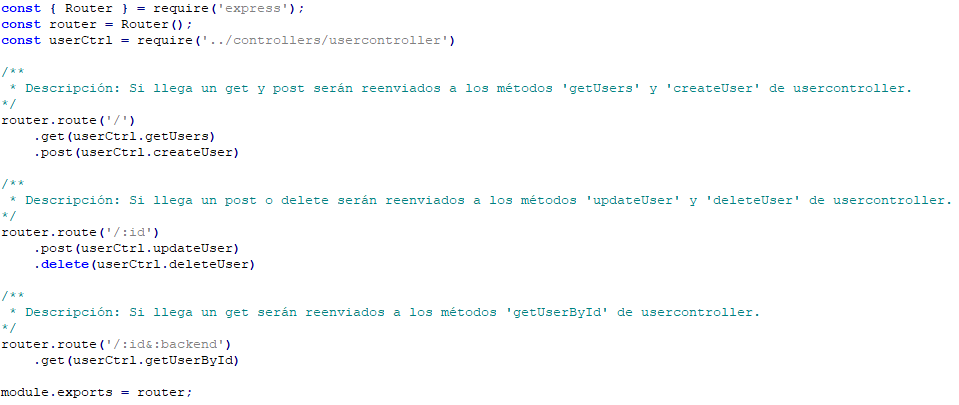
\includegraphics[width=.80\textwidth]{capitulos/capitulo8/routeuser.png}
    \caption{Rutas del usuario.}
    \label{fig:routes}
\end{figure}

Si se envía una petición POST sin parámetros en la URL a la ruta anterior, la petición se va a reenviar al método “createUser()” de los controles de usuario.

\subsection{Controles}
Es la siguiente capa a las rutas. En esta capa se guardan todos los diferentes métodos que gestionan el obtener, añadir, modificar o eliminar datos de la base de datos. Con ayuda de estos controladores se puede hacer cualquier gestión sobre la base de datos. Una vez que la petición ha sido redireccionada en la ruta a uno de los métodos que hay en esta capa, éste se ejecuta y hace las gestiones necesarias.

En el ejemplo nos ha redireccionado una petición POST al método “createUser()”. Una vez que se ejecute este método, la idea es crear un usuario con los datos que nos viene en la petición POST que proviene desde el front-end. Se puede ver el método en la Figura \ref{fig:controller}.

\begin{figure}[h] 
    \centering
    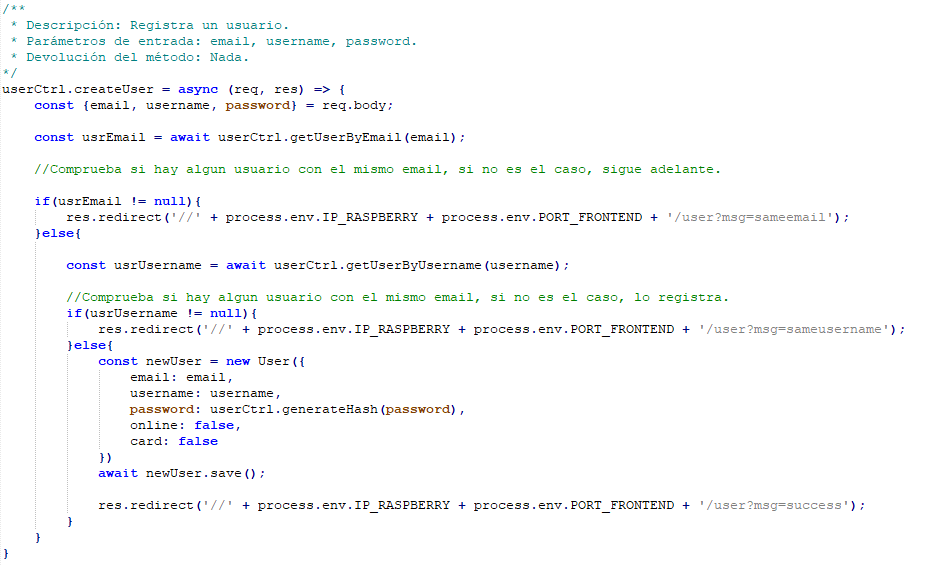
\includegraphics[width=.80\textwidth]{capitulos/capitulo8/usercontroller.png}
    \caption{Método createUser().}
    \label{fig:controller}
\end{figure}

Para ello, se va a obtener el email, nombre de usuario y contraseña de la petición y comprobar si existe algún usuario con ese email. Si existe, se envía un aviso al front-end y no se crea. Se va a hacer lo mismo con el nombre de usuario. 

Si pasa los dos filtros y no existe ningún usuario con ese nombre y correo, se registra el usuario en la base de datos, encriptando la contraseña de éste para mayor seguridad, y se contesta a la petición con un mensaje de que el usuario ha sido creado con éxito.

Al crear el usuario se ha considerado un objeto 'User', donde se guardan los datos de todos los usuarios. Se trata, por tanto, de la base de datos. Hay que recordar que no es una base de datos relacionada, por lo que no está constituida por tablas, sino por objetos. El objeto 'User' se encuentra en la última capa.

\subsection{Objetos}
Es la última capa del back-end. Es la base de datos, donde se guarda la información, y existe un objeto para cada información diferente que guardar. Para el usuario existe el objeto 'User', y en éste se especifican los parámetros que debe de obtener un usuario. Se puede ver el modelo de un objeto usuario en la Figura \ref{fig:object}.

\begin{figure}[h] 
    \centering
    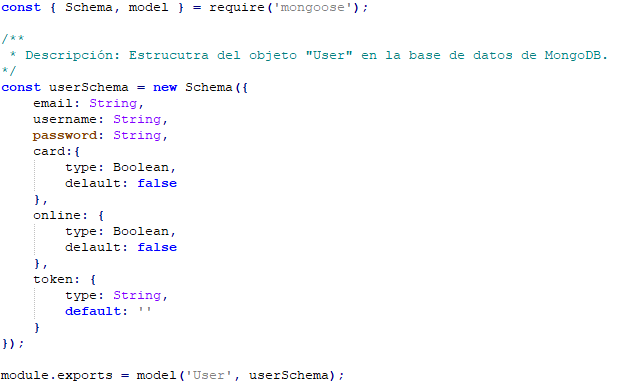
\includegraphics[width=.80\textwidth]{capitulos/capitulo8/modeluser.png}
    \caption{Objecto usuario.}
    \label{fig:object}
\end{figure}

Como se puede apreciar, debe de tener un email, nombre de usuario y contraseña. También va a tener un parámetro llamado ‘card’ y ‘online’ de tipo booleano que por defecto van a estar a false, y un último parámetro llamado 'token' que por defecto va a estar vacío. Los parámetros 'email', 'username' y 'password' sirven para identificar al usuario, el parámetro 'card' es para saber si existe alguna tarjeta RFID asignada a ese usuario, 'online' permite saber si ese usuario está identificado mediante RFID en el sistema, y finalmente 'token' que es para guardar la clave de recuperación usada por si el usuario necesita recuperar su contraseña.

\section{Desarrollo del front-end}
El front-end del sistema es la parte que esta formada por la interfaz, la parte que es vista por el usuario y utiliza para interaccionar con el sistema de una forma visual. Éste se encuentra alojado en la Raspberry, y para acceder a ella hay que utilizar el puerto 3000.

La interfaz está dividida en diferentes páginas, a nivel interno estas páginas se llaman componentes. En total hay 15 páginas diferentes en toda la interfaz.

\subsection{Componentes}
Como se mencionó anteriormente, existen 15 páginas diferentes en toda la interfaz. Los componentes son las siguientes:

\begin{itemize}
    \item \textbf{Login:} Es la página que se ve cuando accedes a la interfaz y no hay ningún usuario logueado. Desde esta página se puede loguear y acceder a las funciones del sistema, o acceder a una página para recuperar la contraseña de un usuario si se le ha olvidado.
    
    \item \textbf{Forget:} Se utiliza para recuperar la contraseña de un usuario que se le ha olvidado. En esta página existe un formulario donde se pide el correo/nombre del usuario a recuperarla. Al introducirlo, el sistema enviará un correo con una clave de seguridad al usuario y reenviará al usuario al componente ‘Recover’.
    
    \item \textbf{Recover:} Se utiliza para recuperar la contraseña de un usuario que se le ha olvidado. En esta página existe un formulario donde se pide la clave de seguridad que se ha enviado al correo, y la nueva clave. Al introducirlo todo, si está correcto, el sistema cambiará la contraseña del usuario y mostrará un mensaje de éxito. Si ha habido algún error, también se mostrará por mensaje.
    
    \item \textbf{Products:} Se visualizan todos los productos que hay dentro del frigorífico ordenados por categorías, también se puede ver la cantidad de cada producto. Solo puede accederse con un usuario logueado. También se puede añadir un producto nuevo a través de un formulario o borrar un producto haciendo clic en el botón de eliminar debajo de cada producto, o hasta editar un producto y el sistema nos reenviará al componente ‘EditProduct’.
    
    \item \textbf{EditProduct:} Solo se puede acceder con un usuario logueado. Aparece un formulario con los datos del producto a modificar. El usuario puede modificar los parámetros que desee y guardar. Si todo se edita correctamente, el sistema devuelve un mensaje de éxito. Si no se edita, se devuelve un mensaje con el error.
    
    \item \textbf{Labels:} Se visualizan todas las etiquetas que hay preparadas para añadir a productos. Se puede ver la cantidad de cada etiqueta. Solo puede accederse con un usuario logueado. También se puede añadir una etiqueta nueva a través de un formulario o borrar una haciendo clic en el botón de eliminar debajo de cada producto, o hasta editar una etiqueta y el sistema nos reenviará al componente ‘EditLabel’.
    
    \item \textbf{EditLabel:} Solo se puede acceder con un usuario logueado. Aparece un formulario con los datos de la etiqueta a modificar. El usuario puede modificar los parámetros que desee y guardar. Si todo se edita correctamente, el sistema devuelve un mensaje de éxito. Si no se edita, se devuelve un mensaje con el error.
    
    \item \textbf{ShoppingList:} Es una página que solo se puede acceder con un usuario logueado. En ella se pueden visualizar los productos que están en la lista de la compra porque la cantidad están por debajo del umbral especificado por el administrador.
    
    \item \textbf{Activity:} Es una página que solo se puede acceder con un usuario logueado. En ella se pueden visualizar la actividad del usuario logueado, con los productos consumidos en un día en específico. También se puede borrar la actividad completa.
    
    \item \textbf{Diet:} Es una página que solo se puede acceder con un usuario logueado. En ella se pueden visualizar la dieta a seguir del usuario logueado, con los productos a consumir en un día en específico y la cantidad de éste. Cada día se enviará un mensaje a cada usuario recordando la dieta a seguir. También se avisará si una dieta no se ha completa, se enviará un mensaje recordando que productos no se han consumido.
    
    Se puede añadir un producto a una dieta de un usuario en un día en específico a través de un formulario. También se puede eliminar un producto ya añadido o editarlo haciendo clic en los respectivos botones.
    
    \item \textbf{EditDiet:} Solo se puede acceder con un usuario logueado. Aparece un formulario con los datos del producto de la dieta a modificar. El usuario puede modificar los parámetros que desee y guardar. Si todo se edita correctamente, el sistema devuelve un mensaje de éxito. Si no se edita, se devuelve un mensaje con el error.
    
    \item \textbf{Users:} Se visualizan todos los usuarios que hay en el sistema. Solo puede accederse con un usuario logueado como administrador. También se puede añadir un usuario nuevo a través de un formulario o borrar un usuario haciendo clic en el botón de eliminar al lado de cada usuario. Otras opciones disponibles es la de añadir un usuario a una tarjeta RFID, o quitar un usuario de una tarjeta. También se puede editar un usuario y el sistema nos reenviará al componente ‘EditUser’.
    
    \item \textbf{EditUser:} Solo se puede acceder con un usuario logueado como administrador. Aparece un formulario con los datos del usuario a modificar. El usuario puede modificar los parámetros que desee y guardar. Si todo se edita correctamente, el sistema devuelve un mensaje de éxito. Si no se edita, se devuelve un mensaje con el error.
    
    \item \textbf{Variable:} Es una página accesible solo por un usuario administrador y en ella se pueden cambiar las variables del sistema, como la variable que identifica el umbral para añadir un producto a la lista de la compra.
    
    \item \textbf{Database:} Es una página accesible solo por un usuario administrador y en ella se pueden limpiar los diferentes objetos de la base de datos.
\end{itemize}

\subsection{Versión móvil/tablet}
El sitio web desarrollado está adaptado para todo tipo de dispositivos móviles y tablets. Así, la funcionalidad es la misma independientemente del dispositivo que el usuario desee. Durante el desarrollo del front-end en primer lugar se realizó enfocado a PC, sin embargo, se vio la necesidad de adaptarlo a dispositivos portátiles. Al realizar esta adaptación, no hubo que rehacer el trabajo que se había realizado anteriormente, sino que se tuvieron que definir estilos adaptados al tamaño de la ventana en la cual se muestra el sistema.

El framework para el front-end que se usa es Bootstrap. Este framework proporciona un conjunto de clases CSS que se asignan a los elementos HTML que se visualizan en el navegador, proporcionando un estilo predefinido. De igual forma, este framework ofrece las herramientas necesarias para hacer adaptables los elementos a los distintos dispositivos.

Al usar Bootstrap, el front-end se divide en 12 columnas, todas ellas de igual tamaño. Así, los elementos pueden definirse para que ocupen las columnas que se desee. Para adaptar el front-end a versión móvil, a medida que se reduzca el tamaño, se tiene que aumentar el número de columnas que ocupa cada elemento para que los elementos que están situados dentro de éste se visualicen correctamente. Además, Bootstrap proporciona un conjunto de tags que se pueden asignar en la clase de un elemento para definir el número de columnas que ocupa éste en cada tamaño de la pantalla (Figura \ref{fig:bootstrap}). De esta manera, utilizando diferentes tags se puede definir cuántas columnas debe utilizar un elemento, dependiendo del tamaño de la pantalla del dispositivo que el usuario esté utilizando.

En el Anexo I se muestran las que se corresponden con la versión móvil del sistema junto con su visualización correspondiente en la versión de ordenador.

\begin{figure}[h] 
    \centering
    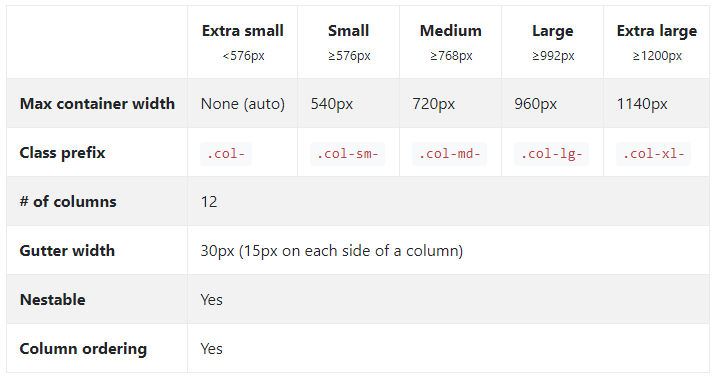
\includegraphics[width=.70\textwidth]{capitulos/capitulo8/boot.png}
    \caption{Uso de las columnas en Bootstrap.}
    \label{fig:bootstrap}
\end{figure}

\section{Despliegue}

Para poder ejecutar el sistema, sin contar con la parte de los sensores y los controladores, primero se debe de descargar todo el contenido software desde el GitHub del proyecto (\url{https://github.com/alexgaro5/SmartFridge}).

A continuaciones se debe de descargar MongoDB (\url{https://www.mongodb.com/download-center/community}) y NodeJS (\url{https://nodejs.org/es/download/current/}).

Finalmente, al abrir el proyecto, en la carpeta raíz (Figura \ref{fig:rootproyect}) se va a encontrar unos ejecutables para desplegar los servidores que crean la comunicación entre los controladores y el back-end, un ejecutable para ejecutar el back-end y otro para el front-end. Haciendo clic en ellos se puede ejecutar lo que se desee.

También hay que recordar que todo el proyecto viene predefinido con unas IPs y puertos por defecto. Se debería de cambiar en las variables de entorno en caso de usar otra configuración de red, situadas en los archivos “.env” del proyecto.

\begin{figure}[h] 
    \centering
    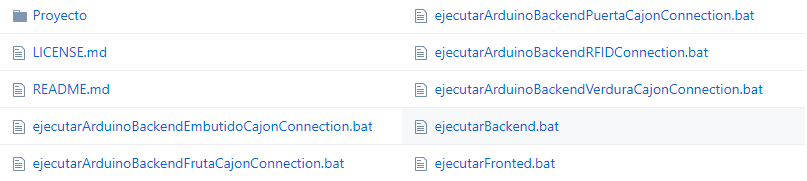
\includegraphics[width=\textwidth]{capitulos/capitulo8/proyect.png}
    \caption{Carpeta raíz del proyecto.}
    \label{fig:rootproyect}
\end{figure}